\section{旋转建模法}
\subsection{绘制左视图}
\begin{procedure}
\item 设置图层,新建“中心线”和“实线”两个图层,具体设计请参看\ref{sec:dianpian}节的图层设置相关内容。
\item  切换视图为主视图。【视图】菜单中【三维视图】子菜单中的【左视图】。
\item 绘制中心线,其结果如图\ref{fig:dianpiancenterline1}所示。
\begin{lstlisting}
|命令: xline|
|指定点或 [水平(H)/垂直(V)/角度(A)/二等分(B)/偏移(O)]:|
|指定通过点:$@1<0$|
|指定通过点:$@1<90$|
|指定通过:|
|命令:OFFSET|
|当前设置: 删除源=否  图层=源  OFFSETGAPTYPE=0|
|指定偏移距离或 [通过(T)/删除(E)/图层(L)] $<$通过$>$:  42|
|选择要偏移的对象,或 [退出(E)/放弃(U)] $<$退出$>$:|
|指定要偏移的那一侧上的点,或 [退出(E)/多个(M)/放弃(U)] $<$退出$>$:|
|选择要偏移的对象,或 [退出(E)/放弃(U)] $<$退出$>$:
\end{lstlisting}
\item 将图层切换为实线层
\begin{figure}[htbp]
\centering
\subfloat[]{\label{fig:dianpiancenterline1}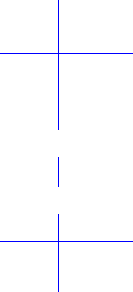
\includegraphics[scale=0.6]{dianpiancenterline1.png}}\hspace{40pt}
\subfloat[]{\label{fig:dianpianleft1}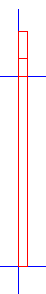
\includegraphics[scale=0.6]{dianpianleft1.png}}
\caption{垫片左视图绘制}
\end{figure}
\item 使用【矩形】命令绘制左视图中的关键特征,其结果如图\ref{fig:dianpianleft1}所示。【矩形】命令的启动方法有:
\begin{itemize}
\item 键盘输入RECTANGLE或REC
\item 点击【绘图】菜单中的【矩形】项。
\item 点击【绘图】工具栏中的【矩形】图标
\includegraphics[scale=0.6]{rectangletool.png}
\end{itemize}
\begin{lstlisting}
|命令: rectang|
|指定第一个角点或 [倒角(C)/标高(E)/圆角(F)/厚度(T)/宽度(W)]:|
|指定另一个角点或 [面积(A)/尺寸(D)/旋转(R)]: @2,52|
|命令: rectang|
|指定第一个角点或 [倒角(C)/标高(E)/圆角(F)/厚度(T)/宽度(W)]:|
|指定另一个角点或 [面积(A)/尺寸(D)/旋转(R)]: @2,4|
|命令: rectang|
|指定第一个角点或 [倒角(C)/标高(E)/圆角(F)/厚度(T)/宽度(W)]:|
|指定另一个角点或 [面积(A)/尺寸(D)/旋转(R)]: @2,26.5|
\end{lstlisting}
\end{procedure}

\subsection{旋转构建垫片的三维模型}
\begin{procedure}
\item 通过建模中的【旋转】操作产生两个圆柱。
\begin{lstlisting}
|命令: REVOLVE|
|当前线框密度:  ISOLINES=4,闭合轮廓创建模式 = 实体|
|选择要旋转的对象或 [模式(MO)]: 找到 1 个|
|选择要旋转的对象或 [模式(MO)]:|
|指定轴起点或根据以下选项之一定义轴 [对象(O)/X/Y/Z] $<$对象$>$:|
|指定轴端点:|
|指定旋转角度或 [起点角度(ST)/反转(R)/表达式(EX)] $<360>$:|
|命令:  REVOLVE|
|当前线框密度:  ISOLINES=4,闭合轮廓创建模式 = 实体|
|选择要旋转的对象或 [模式(MO)]: 找到 1 个|
|选择要旋转的对象或 [模式(MO)]:|
|指定轴起点或根据以下选项之一定义轴 [对象(O)/X/Y/Z] $<$对象$>$:|
|指定轴端点:|
|指定旋转角度或 [起点角度(ST)/反转(R)/表达式(EX)]$ <360>$:|
\end{lstlisting}
\item 关闭“中心线”图层。
\item 切换视图为西南等轴测图。点击【视图】菜单中【三维视图】子菜单中的【西南等轴测】。切换后的结果如图\ref{fig:3darray}所示。
\begin{figure}[htbp]
\centering
\subfloat[]{\label{fig:3darray}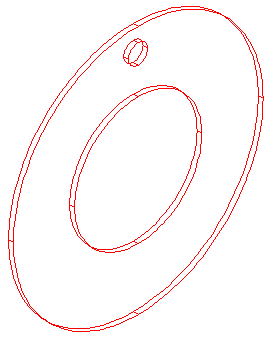
\includegraphics[scale=0.5]{3darray.png}}\hspace{30pt}
\subfloat[]{\label{fig:3darrayselect}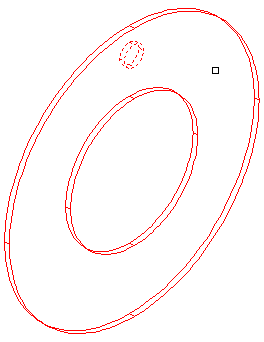
\includegraphics[scale=0.5]{3darrayselect.png}}\hspace{30pt}
\subfloat[]{\label{fig:3darrayresult}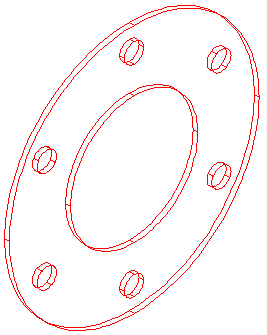
\includegraphics[scale=0.5]{3darrayresult.png}}
\caption{三维阵列过程}
\end{figure}
\item 用【三维阵列】命令阵列$\diameter 8$的圆柱,其结果如图\ref{fig:3darrayresult}所示。启动【三维阵列】命令的方法有:
\begin{itemize}
\item 键盘输入3DARRAY
\item 点击【修改】菜单【三维操作】子菜单中的【三维阵列】项。
\item 点击【建模】工具栏中的【三维阵列】图标
\includegraphics[scale=0.6]{3darraytool.png}
\end{itemize}
\begin{lstlisting}
|命令: 3darray|
|选择对象: 找到 1 个\longremark{选择$\diameter 8$圆柱,如图\ref{fig:3darrayselect}所示。}|
|选择对象:|
|输入阵列类型 [矩形(R)/环形(P)]$<$矩形$>$:p|
|输入阵列中的项目数目: 6|
|指定要填充的角度 (+=逆时针, -=顺时针)$ <360>$:|
|旋转阵列对象? [是(Y)/否(N)] $<Y>$:|
|指定阵列的中心点:\longremark{选择$\diameter 104$圆柱的后底圆圆心。}|
|指定旋转轴上的第二点:\longremark{选择$\diameter 104$圆柱的后底圆圆心。}|
\end{lstlisting}
\showremarks
\item 用差集操作完成垫片的三维建模操作。
\begin{lstlisting}
|命令: subtract |
|选择要从中减去的实体、曲面和面域...|
|选择对象: 找到 1 个|
|选择对象:  选择要减去的实体、曲面和面域...|
|选择对象: 找到 1 个|
|选择对象: 找到 1 个,总计 2 个|
|选择对象: 找到 1 个,总计 3 个|
|选择对象: 找到 1 个,总计 4 个|
|选择对象: 找到 1 个,总计 5 个|
|选择对象: 找到 1 个,总计 6 个|
|选择对象: 找到 1 个,总计 7 个|
|选择对象:|
\end{lstlisting}
\item 设置视觉样式为真实,其结果如图\ref{fig:dianpiansolid}所示。设置方法为:点击【视图】菜单中【视觉样式】子菜单中的【真实】项。
\item 将垫片模型保存为“调压阀垫片立体图.dwg”。
\end{procedure}

\endinput